150. \begin{figure}[ht!]
\center{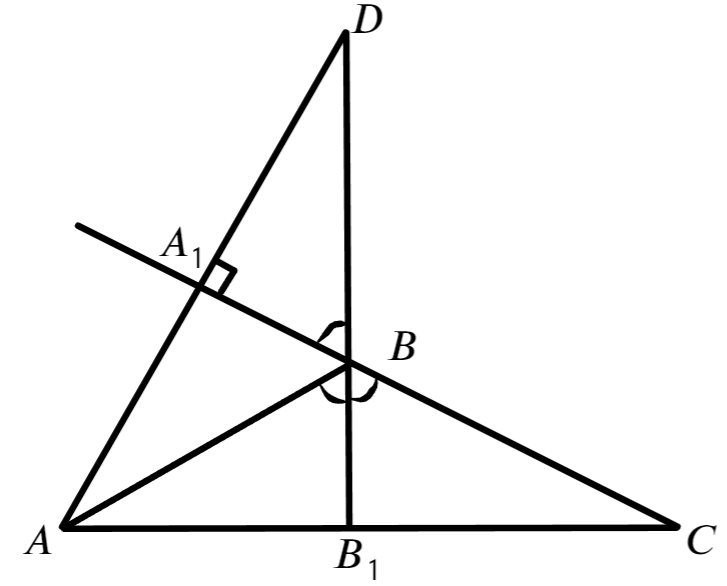
\includegraphics[scale=0.35]{g7-150.png}}
\end{figure}\\
Пусть продолжения высоты $AA_1$ и биссектрисы $BB_1$ пересеклись в точке $D.$ Тогда $\angle DA_1B=90^\circ,\ \angle DBA_1=\angle B_1BC=100^\circ:2=50^\circ$ (так как углы $DBA_1$ и $B_1BC$ вертикальные, а $BB_1$ --- биссектриса). Поэтому $\angle A_1DB=180^\circ-90^\circ-50^\circ=40^\circ.$\\
